\documentclass{tufte-handout}
\usepackage{graphicx}
\usepackage{url}
\usepackage{enumerate}
\usepackage{amsmath,amssymb,amsthm}
\usepackage{enumitem}
\usepackage[iso,american]{isodate}
\usepackage{fancyhdr}
\fancypagestyle{firstpage}{
  \rhead{Creating and Visualizing Curves and Surfaces \linebreak
  \textit{Version: \today}}
}

\title{Creating and Visualizing Curves and Surfaces}
\author{Quantitative Engineering Analysis}
\date{}

\begin{document}

\maketitle
\thispagestyle{firstpage}

\begin{abstract}
\end{abstract}

\section{Overview and Orientation}
We will be thinking about how to define and visualize the surface of a boat, and compute quantities like the displacement, center of mass, center of bouyancy, etc.

\begin{marginfigure}
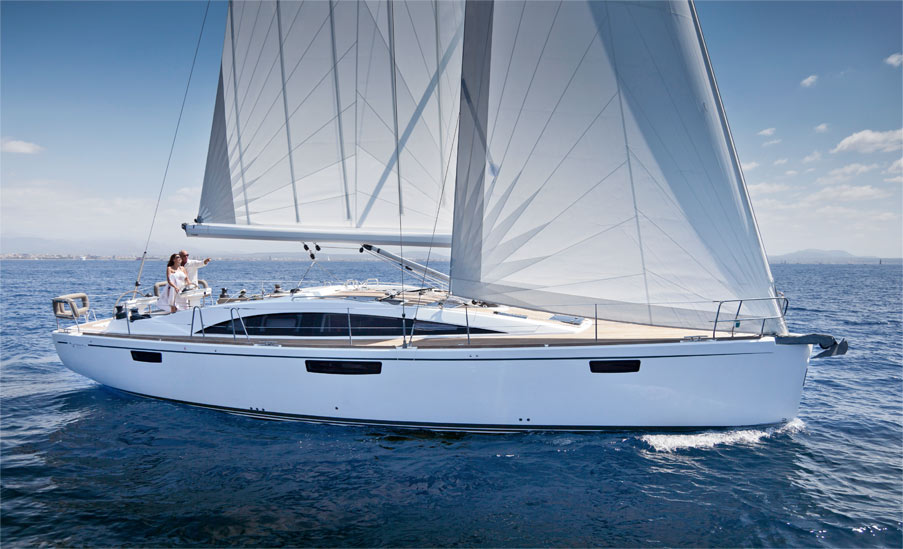
\includegraphics[width=6cm]{figs/bavaria_yacht}
\caption{The great thing about a boat is that it floats, no matter the level of the seas. Credit: bavariayachts.com}
\end{marginfigure}

We need some building blocks about curves and surfaces in order to do this. We will think about functions of several variables, level sets, explicit, implicit, and parametric representations of surfaces, multiple integrals, partial derivatives, Bezier curves and surfaces, elements of CAD.  Some of this will be directly useful for designing a boat, and some of it won't.

The document you are reading constitutes some very brief notes interspersed with a set of exercises. You should plan on reading other sources on your own, and compiling your own notes and ideas. 

\section{Sources}

There is no single book or website that captures all of this material. Some good sources include:

\begin{itemize}
\item Single-variable and Multi-variable calculus. Look for sections on functions, curves and surfaces, partial derivatives, double integrals, triple integrals, parametric curves, parametric surfaces.
\item Computational geometry books, 3D game rendering books, CAD books - look for sections on Bezier curves, Bezier surfaces, B-splines, and NURBS.
\item The articles developed, written, and nurtured by Eric Weisstein at Wolfram Mathworld are a great starting point: mathworld.wolfram.com.
\item Wikipedia is rarely a useful source, at least to begin with, as the quality of entries on technical material is highly variable.
\end{itemize}

\section{Technology}

We will use a variety of technology as we learn more about curves and surfaces. Working on paper or boards is a useful skill, especially for rapid communication between team members. A computer algebra system like {\it Mathematica} (we now have a site license) or {\it Wolframalpha} is an invaluable tool for performing analytical calculations and creating sophisticated visualizations. A numerical computation environment like {\it Matlab} allows us to calculate without algebra, especially when we are dealing with data. Finally, a CAD environment like {\it Solidworks} is critical in developing highly finished products that can then be manufactured. We expect you to use all of these technologies. We don't expect you to be an expert, and we will help you.

For the purposes of this packet, you'll probably find that {\it Wolframalpha} or {\it Mathematica} are your best options to do the visualization, because we're dealing primarily for analytical functions.  We highly recommend that you read through the documentation on Function Visualization at  {\tt https://reference.wolfram.com} to get a bead on this.

You'll also want to be familiar with how to create a visualization of a surface in {\it Matlab}  using the commands {\tt meshgrid}, {\tt surf}, and {\tt contour}.  So if you are not familiar with those two commands, look them up and play with them a bit.


\section{Sections}

\begin{marginfigure}
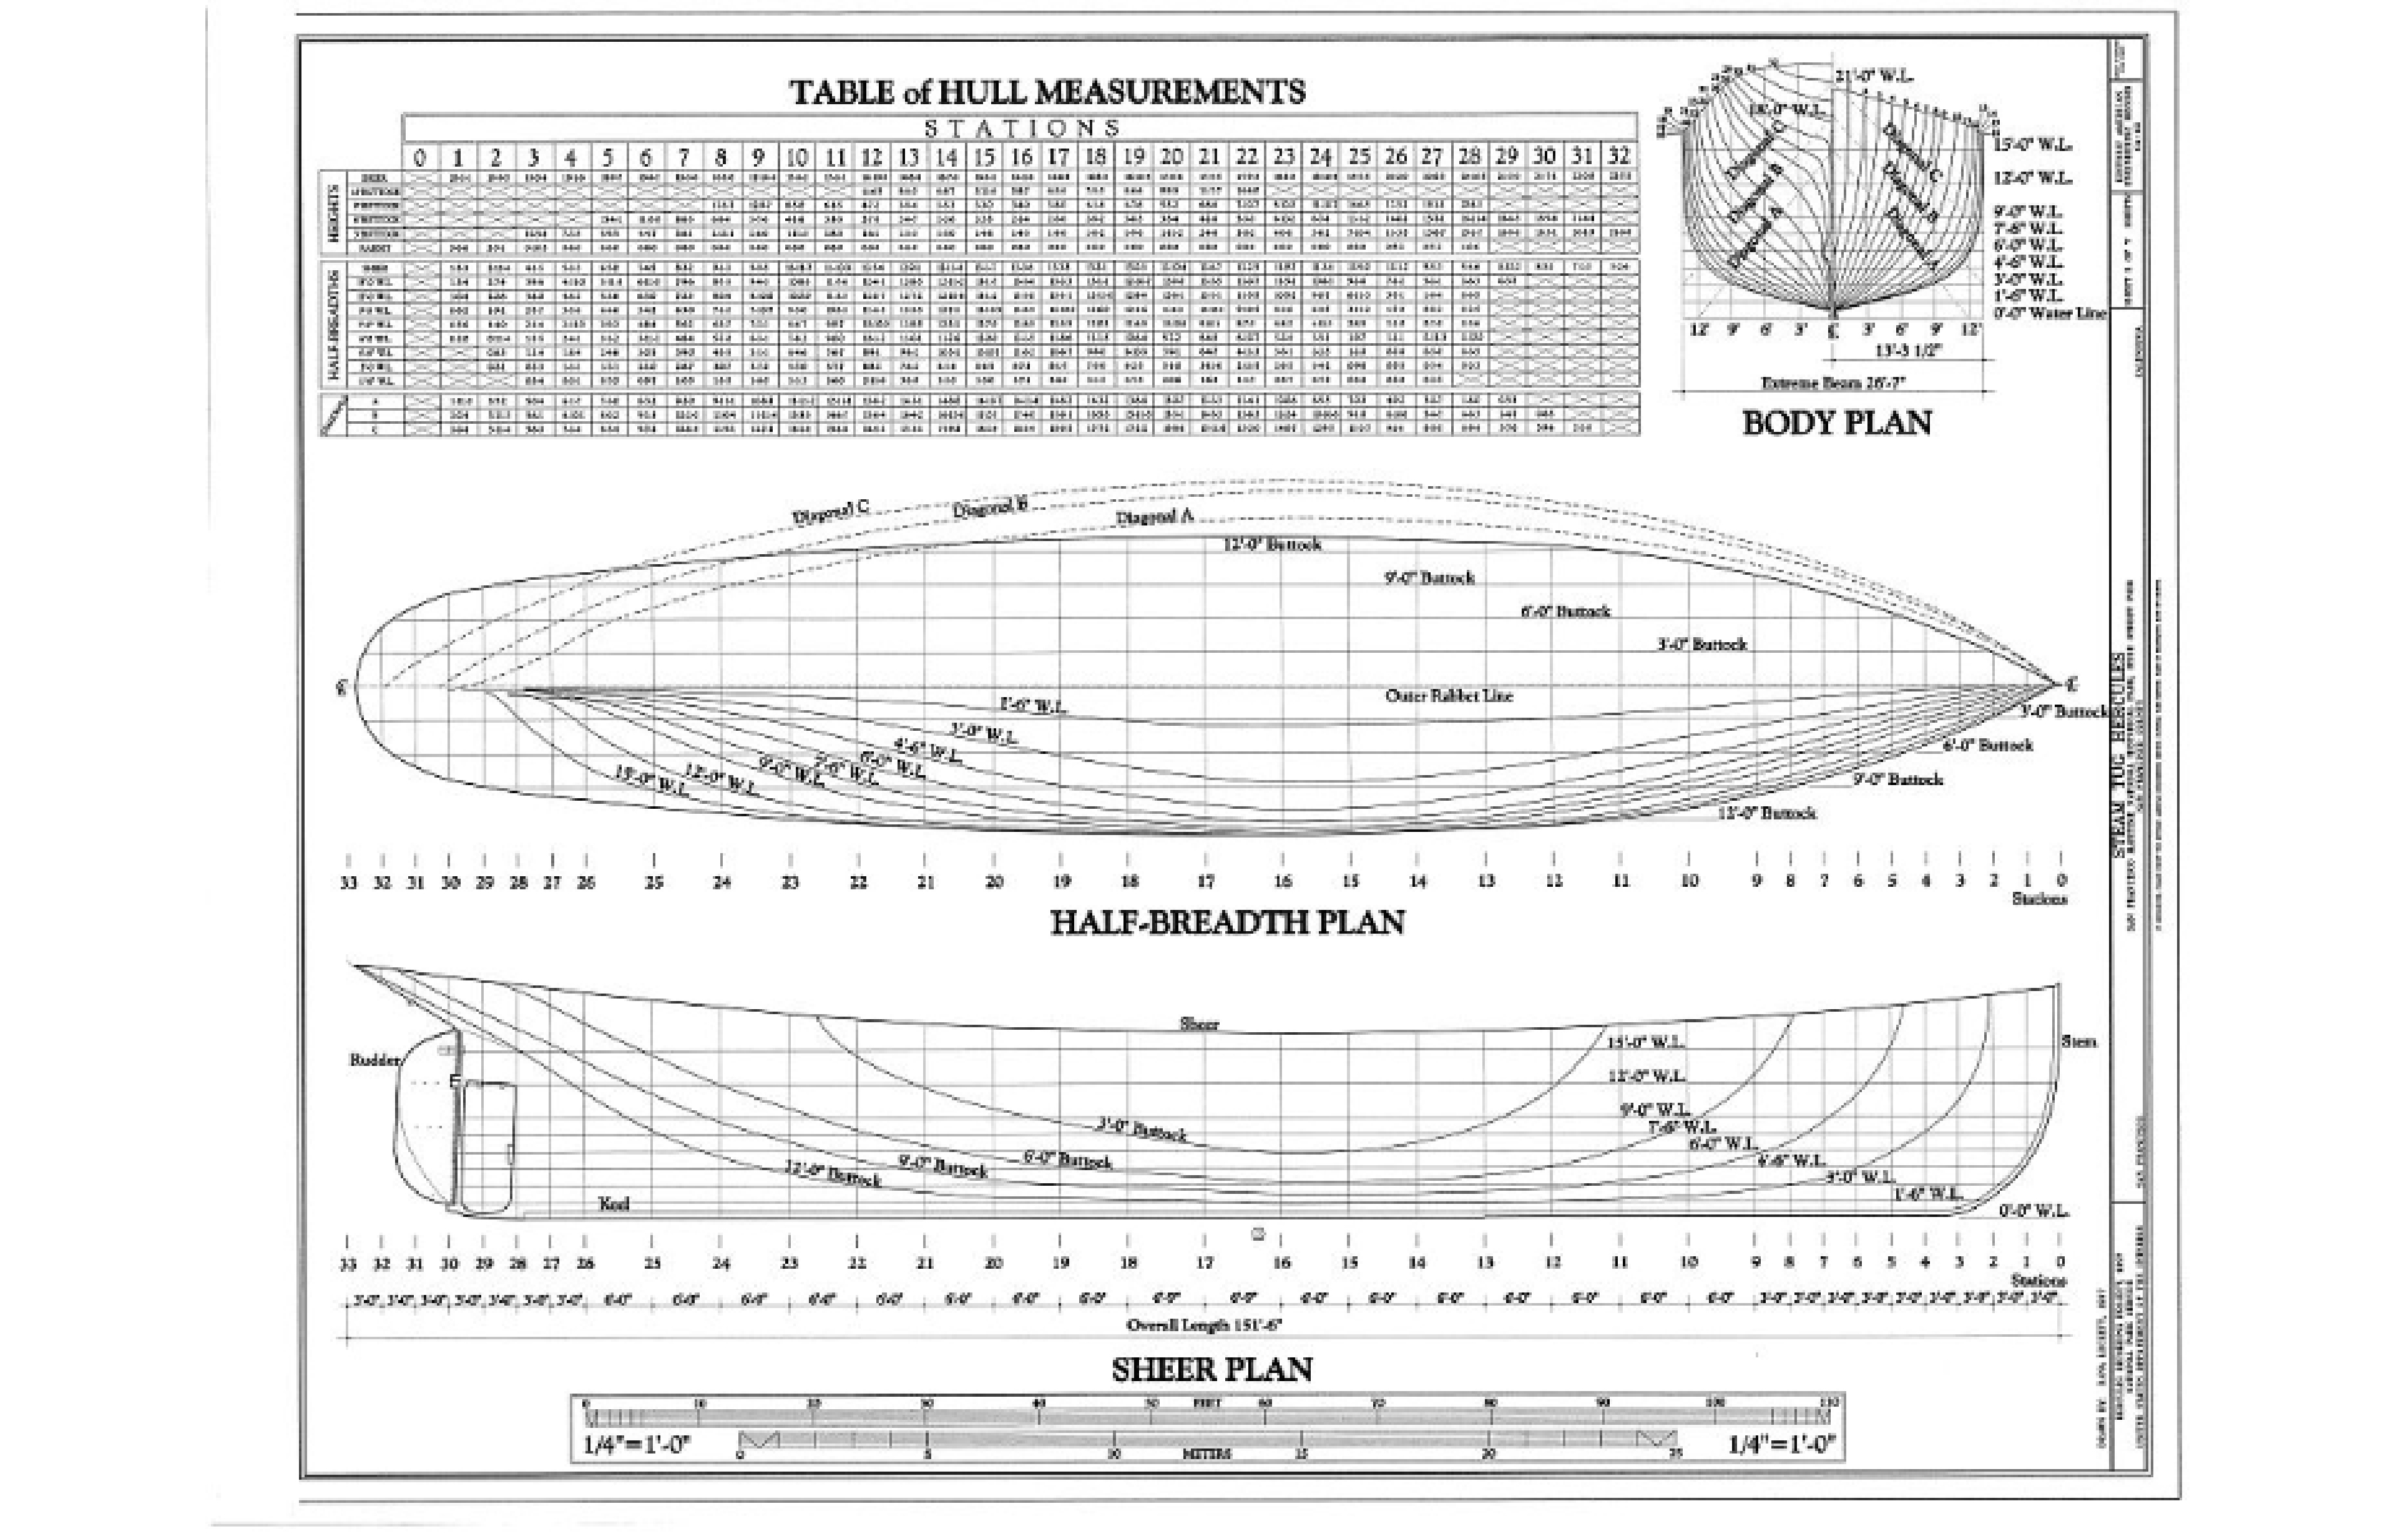
\includegraphics[width=6cm]{figs/hercules_shiplines}
\caption{Stations (top), buttocks and waterlines (w.l.) marked on the plans of the steam tug Hercules. Credit: Library of Congress}
\end{marginfigure}

Let's think about a surface by creating slices through it. There are three common slices used on boats: stations, buttocks, and waterlines. More generally these are called sections. Slices are actually the intersections of a plane with a surface. Slices create regions in cutting plane bounded by curves (a line is a curve). These curves are often called contour levels or level sets. We will use mutually orthogonal slices (or planes) for now.

\begin{enumerate}
\item Pick a fruit or vegetable, slice it in three ways, and sketch the sets of curves defined by each of these sets of slices.
\item Pick a manufactured object, imagine slicing it in three ways, and sketch the set of curves defined by each of these sets of slices.
\item Create a representation of one of these objects by cutting sections out of 1 inch blue foam and glueing them together.
\end{enumerate}

\section{Symmetry}

Many objects have symmetry:  one or more ways that you can manipulate the object where the object looks the same after the manipulation.  Common examples include reflection symmetry across a plane, or rotation symmetry about an axis.  One object may have multiple planes of reflection symmetry and multiple axes of rotation symmetry.  Identifying these symmetries can help in accurately describing an object.

\begin{enumerate}[resume]
\item Identify any reflection or rotation symmetries of your objects.  Sketch your most symmetric object and indicate reflection planes and rotation axes of symmetry.
\end{enumerate}

\section{Coordinates}

Many of the surfaces that we are interested in are embedded in 3D, and we will want to be able to describe these surfaces using a three dimensional coordinate system.  The choice of coordinate system is often determined by the symmetries of your system. At this stage, we will use a Cartesian coordinate system $(x,y,z)$ to describe points on the surface. It should obey the right-hand rule. We are free to place the origin wherever we see fit, and to orient the axes as needed.

\begin{enumerate}[resume]
\item For both the fruit/vegetable and the manufactured object, propose two different origins and orientations of the coordinate system.  What are the pros and cons of each one?
\end{enumerate}

\begin{marginfigure}
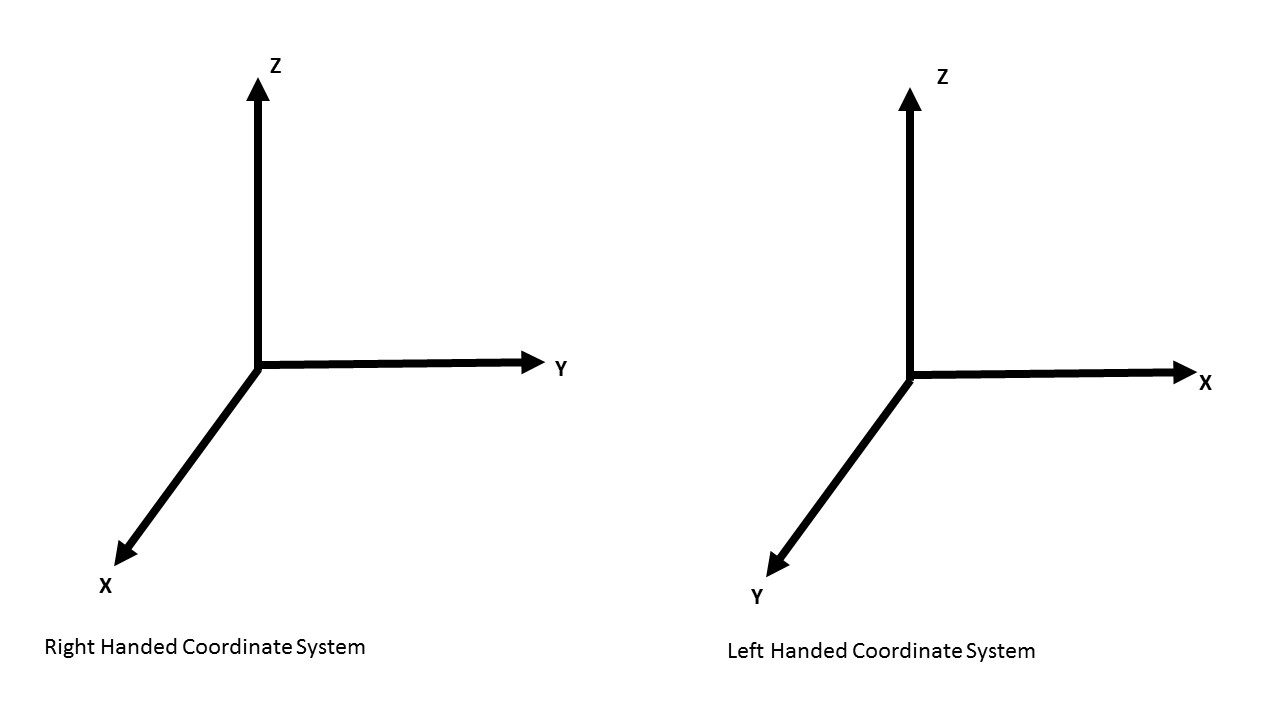
\includegraphics[width=6cm]{figs/LHandRHCoord}
\caption{Right handed and Left handed Cartesian Coordinate Systems.  Note:  If you turn the top of a screw from the x axis toward the y axis, the top of the screw will move up in z.}
\end{marginfigure}

\section{Curves defined explicitly by $y=f(x)$}

All of single-variable calculus involved explicit functions of a single variable, e.g. $y = x^2, y = sin(x)$, or more generally $y = f(x)$. You spent a lot of time visualizing these functions, considering their properties like odd/even symmetry, number of zeros, and periodicity, and computing related properties like derivatives and integrals. Some of these functions are worth having at your fingertip.

\begin{enumerate}[resume]
\item Compile a table of basic, explicit functions. Include their name, a sketch, and a function definition. Your table should include polynomials, trigonometric functions, exponentials and logarithms.
\item Choose a couple of curves that you sketched earlier (fruit, vegetable, object), and propose an explicit function that approximates some section of the curve.  Using either Wolfram Alpha or MATLAB, check that your explicit function looks right.
\end{enumerate}

\begin{marginfigure}
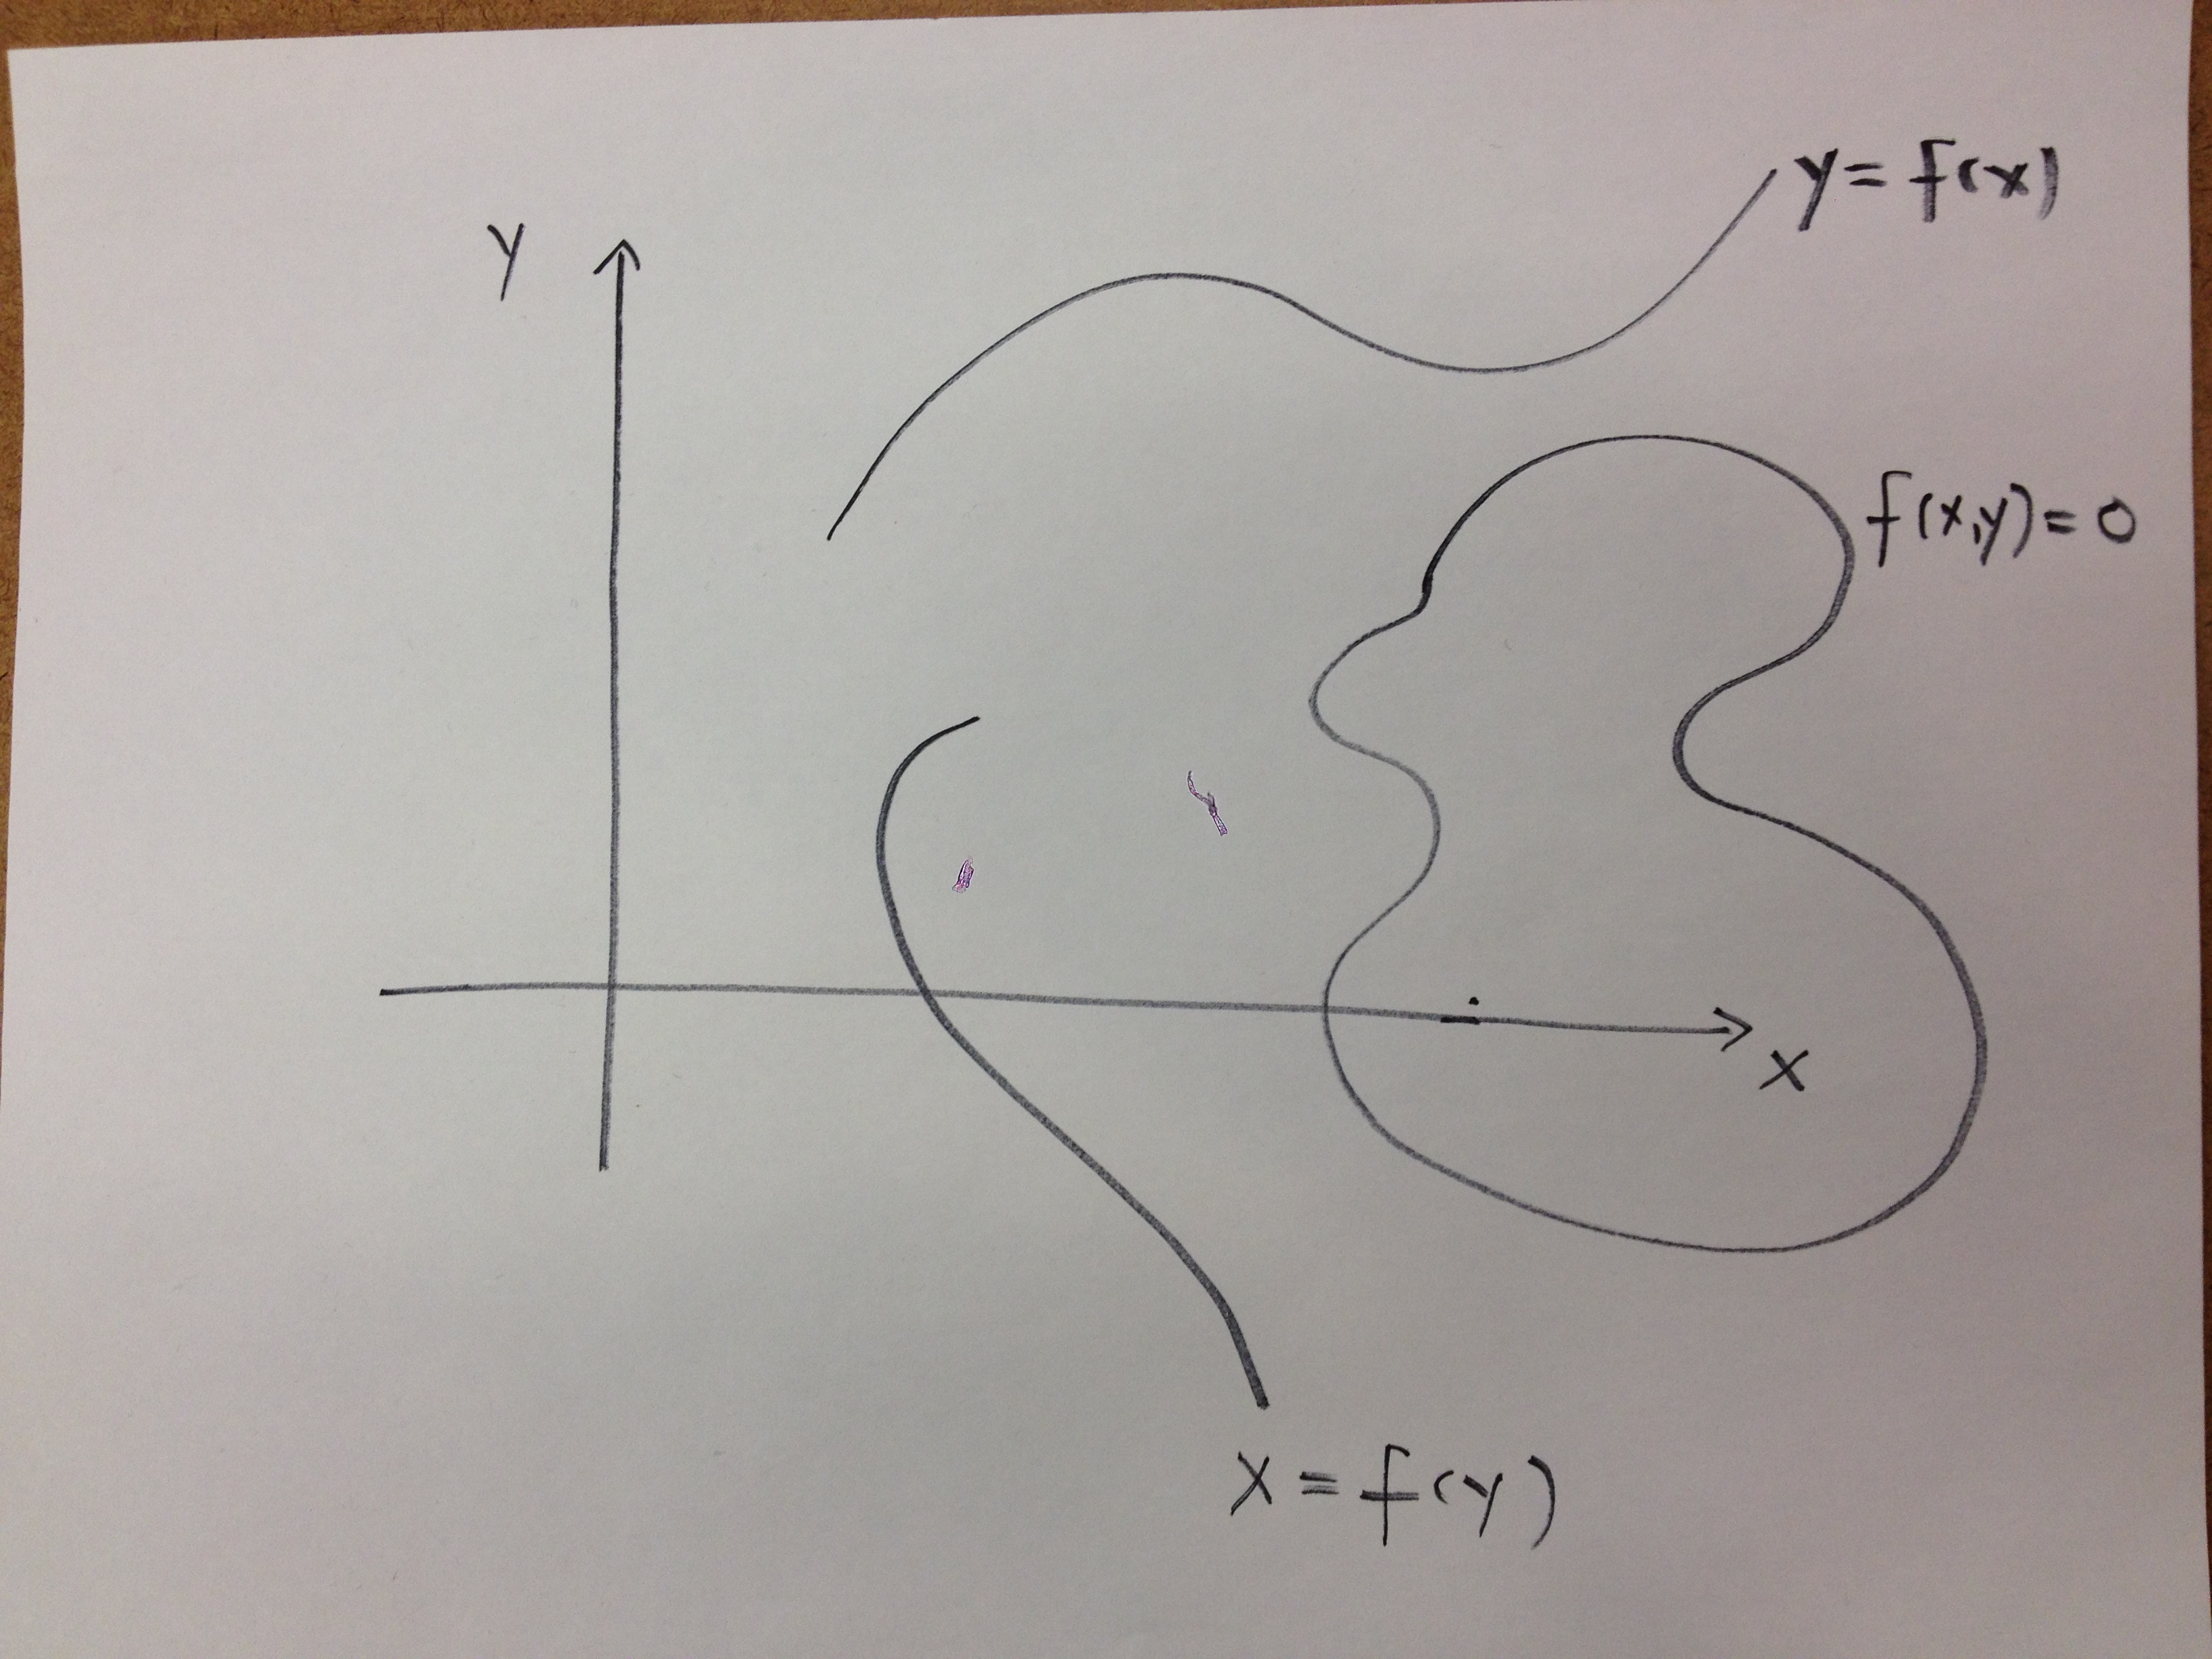
\includegraphics[width=6cm]{figs/curves}
\caption{Curves can be defined explicitly, $y = f(x)$ , $x = f(y)$, or implicitly, $f(x,y)=0$.}
\end{marginfigure}

\section{Curves defined implicitly by $f(x,y)=0$}

Not every curve can be expressed in terms of an explicit function. A circle is a good example. Curves can also be expressed implicitly through a relationship between 2 variables. For example, the equation for a circle of radius $R$, centered at $(x,y)=(a,b)$ is $(x-a)^2 + (y-b)^2 - R^2 = 0$. The left-hand side of this equation can be thought of as a function of two variables,
\[f(x,y) = (x-a)^2 + (y-b)^2 - R^2 \]
and the set of points $(x,y)$ where $f=0$ defines a curve that we like to call a circle.

There is no end to the functions of two variables that you can define. Figuring out the curve defined implicitly by setting $f=0$ is usually a task for a Computer Algebra System. There is, however, a set of functions that show up again and again, and these are the quadratic functions of two variables. The general form (containing all possible quadratic, linear and constant terms) is
\[f(x,y) = Ax^2 + Bxy + Cy^2 + Dx + Ey + F\]
where $A,B,C,D,E,F$ are arbitrary parameters, some of which may be zero. The curves defined by $f=0$ are called conic sections, and represent the intersection of a double cone and a plane. They include lines, planes, circles, parabolas, ellipses, and hyperbolas.

\begin{enumerate}[resume]
\item Review a catalogue of the conic sections. Pick out a couple of your favorites. Name them, sketch them, and write down the implicit function that defines them.
\item Would any of your curves from earlier be better represented with an implicit function? If so, propose one.  
\item If you propose an implicit function to represent one of your curves, visualize that function using the computational tool of your choice. If you did not propose an implicit function, visualize the curve 
\[f(x,y) = x^2 + xy + y^2 - x - y - 1=0\].
\end{enumerate}

\section{Surfaces defined explicitly by $z = f(x,y)$}

If we assign the output of a function of two variables to be a third variable, then the set of points define a surface. For example, $z = x^2 + y^2$ is a paraboloid. Let's cut sections parallel to the $xy$-plane at different values of z. If we let $z=C$ then each section is a circle in the $xy$-plane of radius $\sqrt{C}$. If we cut sections parallel to the $xz$-plane ($y=C$) then each section is a parabola in the $xz$-plane. Finally, if we cut sections in the $yz$-plane ($x=C$) then each section is a parabola in the $yz$-plane. Putting these sections together defines a surface known as a paraboloid.

\begin{marginfigure}
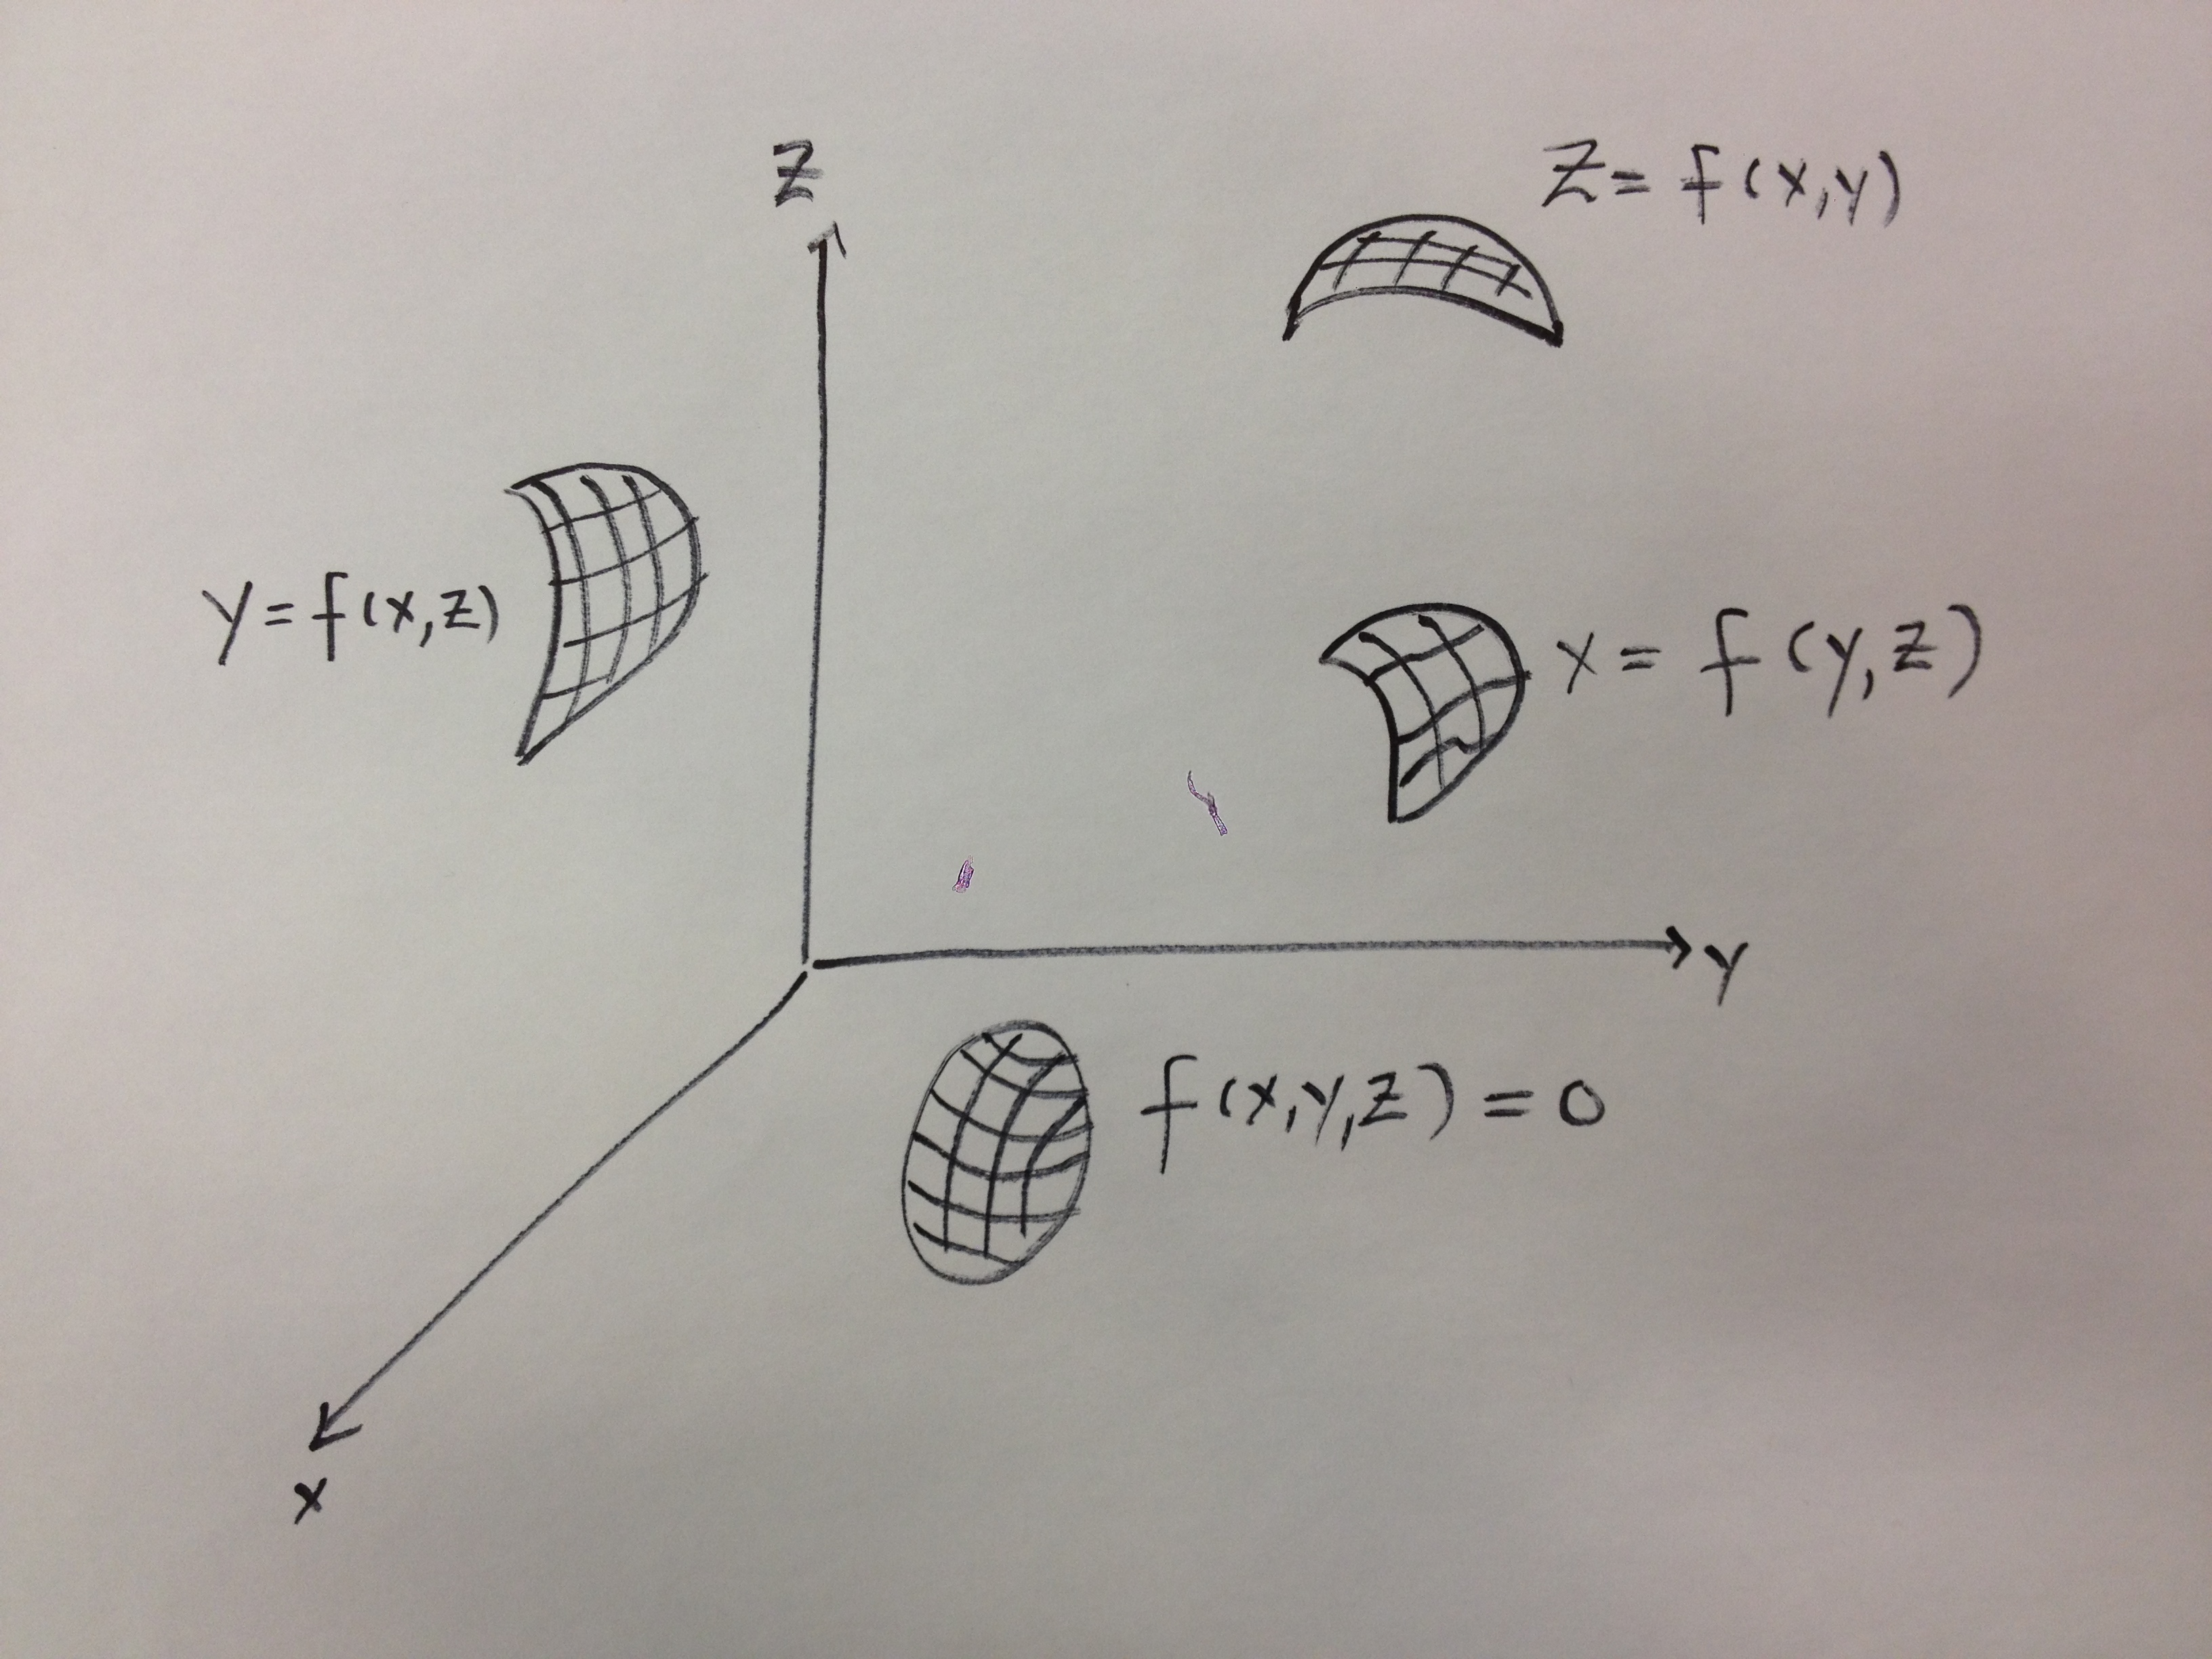
\includegraphics[width=6cm]{figs/surfaces}
\caption{Surfaces can be defined explicitly, $z = f(x,y)$ , $x = f(y,z)$, $y = f(x,z)$, or implicitly, $f(x,y,z)=0$.}
\end{marginfigure}

\section{Surfaces defined implicitly by $f(x,y,z) = 0$}
A surface in three dimensions can also be implicity defined by a function $f(x,y,z) = 0$.  One class of these is the group of quadratic (or quadric) surfaces, defined by the set of functions:
\[f(x,y) = Ax^2 + By^2+ +Cz^2 + Dyz + Ezx+Fxy+Gx+Hy+Iz+J=0\]
where $A,B,C,D,E,F,G,H,I,J$ are all arbitrary constants, some of which may be zero.

\begin{enumerate}[resume]
\item Review a catalogue of the quadratic surfaces. Pick out a couple of your favorites. Name them, sketch them, and write down the function that defines them.
\item Choose a fruit/vegetable or manufactured object and propose an explicit or implicit representation of its surface.
\item Visualize your chosen representation using an appropriate computational tool.
\end{enumerate}

\section{Surfaces defined by sweeping}

Recall the fruit cutting exercise. If the cutting plane was $xz$, then the section curve lies in the $xz$-plane, and may be described by the explicit function $z=f(x)$. If the cutting plane was $yz$, then the section curve may be described by the explicit function $z = g(y)$. A swept surface is formed by sweeping one curve along another curve. This amounts to defining the surface as a product of two section curves, i.e.
\[z = f(x) g(y) \]

% Image of sweeping

\begin{enumerate}[resume]
\item Create approximate surfaces of the fruit/vegetable and manufactured object by sweeping. Plot these in Solidworks. Discuss the ways in which the approximate surfaces fails to match that of the object. If it matches the surface of the object, then please explain why.
\end{enumerate}

See {\it Function Driven Curve} and {\it Swept Surface} in SOLIDWORKS.

\section{Surfaces defined by revolution}

You probably met this idea in single-variable calculus. Rotating a curve about an axis defines a surface of revolution. The curve is called the generatrix and the axis is the axis of rotation. Many natural and manufactured objects have surfaces that can be created this way. Consider a generatrix that lies in the $xy$-plane and is described by $y=f(x)$. Rotating about the x-axis generates a surface with circular section in the $yz$-plane of radius $f^2$. The equation for the surface is therefore
\[y^2 + z^2 = f^2(x) \]
If the generatrix is given in implicit form, $f(x,y) = 0$, then the equation for the surface is
\[f(x,\sqrt{y^2+z^2}) = 0\]

% An example image of revolution here?

\begin{enumerate}[resume]
\item Record and sketch at least five objects (natural or manufactured) which have a surface of revolution or part of one. Identify at least one axis of rotation.
\item Choose one of them and sketch the boundary curve obtained by making an imaginary cut along a plane containing the axis of rotation.
\item Create an explicit function that approximates the boundary curve, and write down the equation that defines the surface of revolution.
\item  Create this surface in Solidworks.
\end{enumerate}

See {\it Revolved Surface} in SOLIDWORKS.

\section{Surfaces defined by lofting}

Lofting refers to the process of building a surface by connecting a set of curves. Consider two boundary curves obtained at $z=0$ and $z=1$. Represent them as $y=f_1(x)$ and $y=f_2(x)$. The lofted surface between these two curves is defined as a linear combination of these two functions, namely
\[y = (1-z) f_1(x) + z f_2(x) \]
where we have assumed that $z \in [0,1]$.

% Do we want an image of lofting here?

\begin{enumerate}[resume]
\item Choose a fruit, vegetable, or manufactured object, and create an approximation to the surface by lofting.
\item  Create this surface in Solidworks.
\end{enumerate}

See {\it Lofted Surface} in SOLIDWORKS.

\end{document} 